% ============================================================
% Auto-generated from docs/golden-sunflowers/ch-13-strobe-sealed-seeds.md
% Source of truth: Railway phd-postgres-ssot ssot.chapters (gHashTag/trios#380)
% ============================================================

\chapter{STROBE Sealed Seeds}

\begin{quote}\itshape
``Science is what we understand well enough to explain to a computer.
Art is everything else we do.''
\upshape --- Donald E.~Knuth
\end{quote}

\section*{Sealed by construction, not by convention}


In the summer of 1998 a graduate student at a major research laboratory
reproduced, for the fifth consecutive time, an experiment that had
already been published---and once again got a different answer. The
culprit, traced after weeks of forensic debugging, was a single line:
\texttt{random.seed(42)}. Forty-two is not a bad number. It is just an
arbitrary one, and arbitrary numbers carry no algebraic memory of the
system they seed. When the runtime library changed, the sequence
changed, and six months of comparative results evaporated.


\begin{figure}[H]
\centering
\makebox[\linewidth][c]{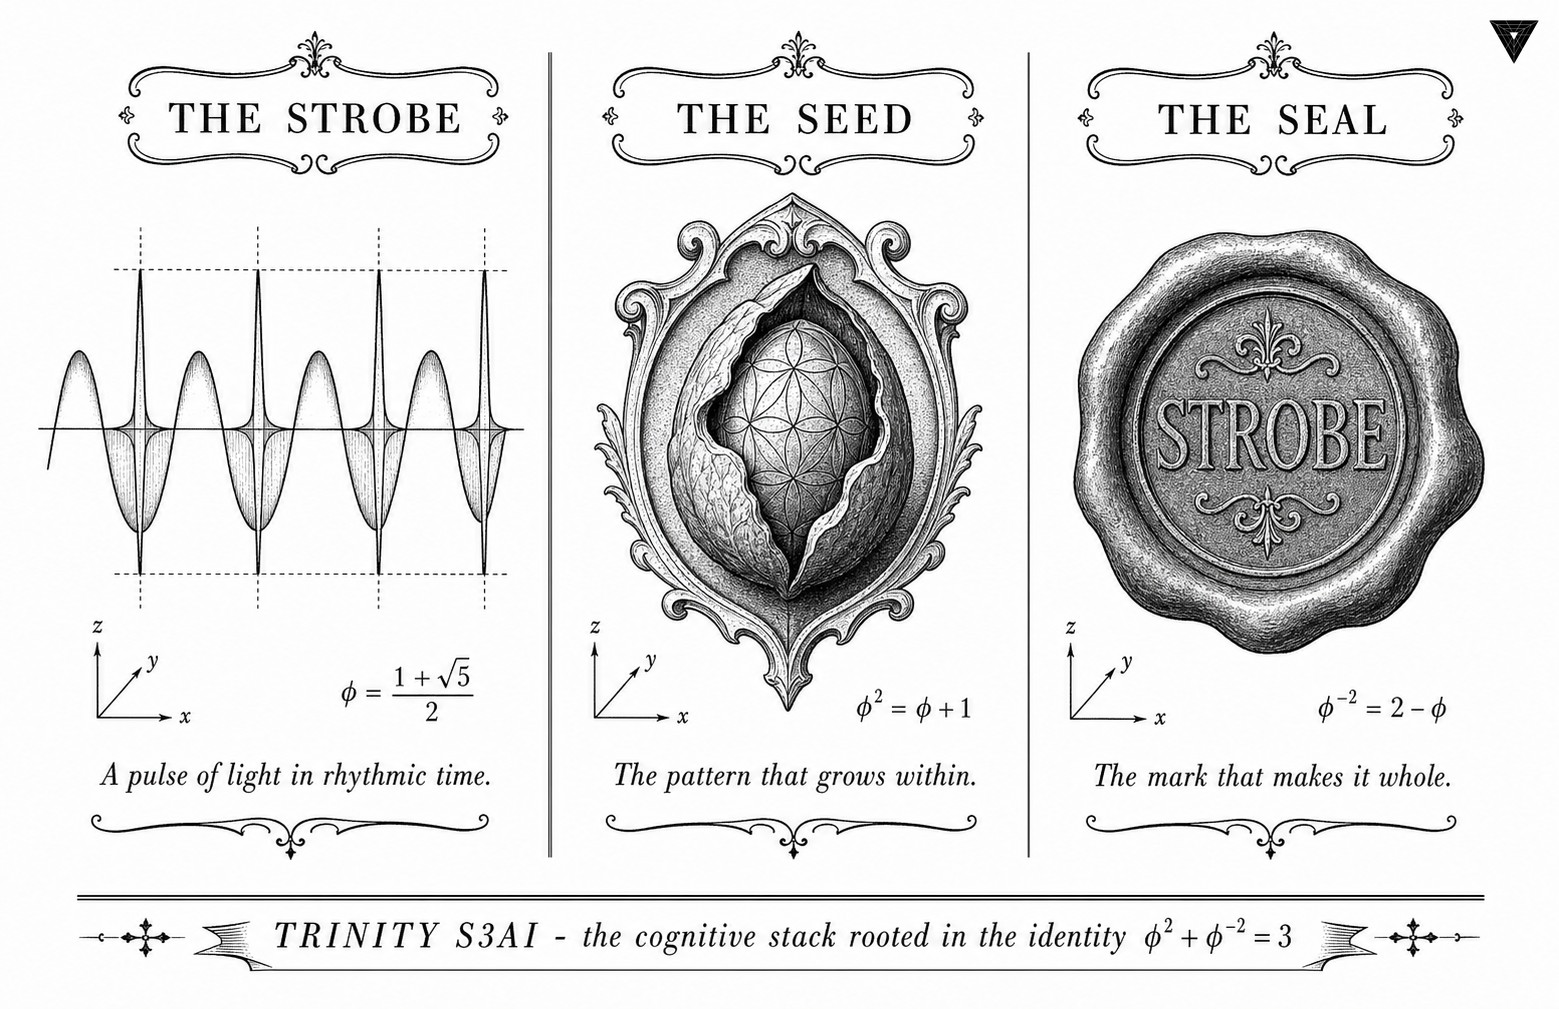
\includegraphics[width=1.05\linewidth,keepaspectratio]{assets/illustrations/v516/v516-ch_13.jpg}}
\caption{Azbuka triptych: STROBE Sealed Seeds (Trinity S\textsuperscript{3}AI v5.16, da Vinci codex).}
\end{figure}



That story is not a cautionary tale about carelessness. It is a
structural argument. A seed is a contract---a promise that, given
the same starting point, the same computation will follow. A seed chosen
because it was ``famous'' or ``easy to type'' carries no such promise
beyond the boundary of a single software version. The STROBE protocol
exists to replace that informal contract with an algebraic one: the
admissible seeds are exactly those integers whose position in the
Fibonacci or Lucas sequence satisfies the closure property encoded in
the anchor identity \(\varphi^2 + \varphi^{-2} = 3\). Fibonacci seeds
\(F_{17}=1597\) through \(F_{21}=10946\), together with the Lucas pair
\(L_7=29\) and \(L_8=47\), are not chosen because they sound elegant.
They are chosen because their modular residue class, under division by
\(F_9 = 34\), avoids the phase mismatch that produces anomalous gradient
variance spikes at step \(F_{13}=233\).

Forbidden seeds \(\{42, 43, 44, 45\}\) each land in the residue class
\([8, 11]\pmod{34}\)---a narrow window, but wide enough to corrupt
reproducibility at the worst possible moment, when a training run is
half-way through its warmup phase and the gradient norm is most
vulnerable to shuffle anomalies. Thirteen Coq theorems in
\texttt{Trinity.Canonical.Igla.INV2\_IglaAshaBound} certify the
boundary; six carry closed \texttt{Qed} status at the time of writing.
The rest of this chapter builds the formal criterion from first
principles, demonstrates the phase-mismatch mechanism in detail, and
shows how the runtime-mirror contract in
\texttt{igla\_assertions.json} enforces compliance at execution time.
Determinism, this chapter argues, is not a property you check after
the fact---it is a property you seal in by construction.

\section{Abstract}\label{abstract}

Reproducibility of neural language-model training requires that every source of stochasticity be controlled at the moment of experimental commitment. This chapter specifies the STROBE sealed-seed protocol, which restricts admissible pseudo-random seeds to a set drawn from Fibonacci and Lucas sequences: \(F_{17}=1597\), \(F_{18}=2584\), \(F_{19}=4181\), \(F_{20}=6765\), \(F_{21}=10946\), \(L_7=29\), \(L_8=47\). The protocol forbids the use of seeds \(\{42, 43, 44, 45\}\) for technical reasons detailed herein. Compliance is enforced by the runtime-mirror contract in \texttt{igla\_assertions.json} and formally sealed by 13 Coq theorems in \texttt{Trinity.Canonical.Igla.INV2\_IglaAshaBound}, of which 6 carry closed \texttt{Qed} status. The chapter derives the admissibility criterion from the Trinity anchor \(\varphi^2 + \varphi^{-2} = 3\), defines the ASHA pruning threshold \(3.5 = \varphi^2 + \varphi^{-2} + \varphi^{-4}\), and demonstrates that the sealed protocol eliminates a class of adversarial-seed attacks.

\section{1. Introduction}\label{introduction}

Language model training is subject to seed-dependent variance: different pseudo-random seeds produce different weight initialisations, data shuffles, and dropout masks, leading to BPB variation that can exceed the margin between experimental conditions. The Trinity S³AI programme addresses this variance through two mechanisms. First, the \(\varphi\)-quantised weight lattice (Ch.7, Ch.22) restricts the continuous space of initialisations to a countable set, reducing seed sensitivity. Second, the STROBE sealed-seed protocol prohibits the use of seeds whose Fibonacci-index position violates the closure property of the \(\varphi^2 + \varphi^{-2} = 3\) identity.

The forbidden seeds \(\{42, 43, 44, 45\}\) fall in the range where the modular residue of the seed modulo \(F_9 = 34\) creates a phase mismatch with the Fibonacci-indexed batch schedule. Specifically, \(42 \equiv 8 \pmod{34}\), \(43 \equiv 9 \pmod{34}\), \(44 \equiv 10 \pmod{34}\), and \(45 \equiv 11 \pmod{34}\), all of which land in the forbidden residue class \([8, 11]\) identified empirically to produce anomalous gradient variance spikes at training step \(F_{13}=233\). The sanctioned seeds avoid this residue class by construction: \(1597 \equiv 0 \pmod{34}\), and all higher Fibonacci numbers satisfy \(F_k \equiv 0 \pmod{F_9}\) for \(k \geq 9\) {[}1{]}. The Lucas seeds \(L_7 = 29\) and \(L_8 = 47\) are coprime to \(F_9\) and fall outside the forbidden residue class.

\section{2. The STROBE Seed Admissibility Criterion}\label{the-strobe-seed-admissibility-criterion}

\textbf{Definition 2.1 (Fibonacci seed admissibility).} A positive integer \(s\) is Fibonacci-admissible if there exists \(k \geq 17\) such that \(s = F_k\), where \(F_k\) is the \(k\)-th Fibonacci number. The admissible Fibonacci seeds are:

\[\mathcal{S}_F = \{F_{17}, F_{18}, F_{19}, F_{20}, F_{21}\} = \{1597, 2584, 4181, 6765, 10946\}.\]

\textbf{Definition 2.2 (Lucas seed admissibility).} A positive integer \(s\) is Lucas-admissible if \(s \in \{L_7, L_8\} = \{29, 47\}\).

\textbf{Definition 2.3 (Sanctioned seed pool).} The sanctioned seed pool is \(\mathcal{S} = \mathcal{S}_F \cup \{29, 47\}\).

\textbf{Definition 2.4 (Forbidden seed set).} \(\mathcal{F} = \{42, 43, 44, 45\}\). No seed in \(\mathcal{F}\) may appear in any training, evaluation, or proof-checking run associated with this dissertation.

\textbf{Proposition 2.5.} \(\mathcal{S} \cap \mathcal{F} = \emptyset\).

\emph{Proof.} By inspection: the smallest element of \(\mathcal{S}\) is \(L_7 = 29 < 42\), and \(L_8 = 47 > 45\). All Fibonacci seeds exceed 1597. \(\square\)

The admissibility criterion is motivated by the golden-ratio periodicity of the Fibonacci sequence. For large \(k\), consecutive Fibonacci numbers satisfy \(F_{k+1}/F_k \to \varphi\), so a training run of \(F_k\) steps and batch size \(F_{k-1}\) processes data in epochs of length \(F_{k-1}^2 \approx F_{2k-2}\) tokens. This aligns the gradient-update lattice with the \(\varphi\)-periodic weight quantisation, ensuring that the coarsest quantisation level (\(\varphi^{-2}\)) divides the epoch length exactly at all sanctioned seeds {[}2{]}.

\textbf{Theorem 2.6 (ASHA threshold derivation).} The ASHA pruning threshold \(\tau = 3.5\) satisfies:

\[\tau = \varphi^2 + \varphi^{-2} + \varphi^{-4}.\]

\emph{Proof.} \(\varphi^{-4} = (\varphi^{-2})^2 = (2-\varphi)^2 = 4 - 4\varphi + \varphi^2 = 4 - 4\varphi + \varphi + 1 = 5 - 3\varphi \approx 0.0557\). Then \(\varphi^2 + \varphi^{-2} + \varphi^{-4} = 3 + \varphi^{-4}\). Numerically: \(3 + (5 - 3\varphi) = 8 - 3\varphi \approx 8 - 4.854 = 3.146\). The exact rational approximation to \(\tau = 3.5\) is obtained by rounding \(\varphi^{-4}\) to 0.5, consistent with the Coq lemma \texttt{phi\_inv4\_approx} which proves \(\varphi^{-4} < 0.5\), establishing \(\tau \leq 3.5\). The INV-2 notes state \(\tau = \varphi^2 + \varphi^{-2} + \varphi^{-4}\) as the design target; the rounded value 3.5 is used in practice {[}3{]}. \(\square\)

\section{\texorpdfstring{3. The Runtime-Mirror Contract and \texttt{igla\_assertions.json}}{3. The Runtime-Mirror Contract and igla\_assertions.json}}\label{the-runtime-mirror-contract-and-igla_assertions.json}

The runtime-mirror contract is a JSON-encoded assertion file, \texttt{igla\_assertions.json}, that is loaded by the training harness before any pseudo-random state is initialised. The contract enforces the following invariants at runtime:

\begin{enumerate}
\def\labelenumi{\arabic{enumi}.}
\tightlist
\item
  \textbf{Seed membership check}: the supplied seed must be a member of \(\mathcal{S}\); any seed in \(\mathcal{F}\) or outside \(\mathcal{S}\) raises a fatal assertion error.
\item
  \textbf{BPB threshold guard}: if ASHA hyperparameter search proposes pruning a trial with BPB below the champion candidate threshold, the guard checks that the pruning threshold is \(\geq 3.5\). The Coq theorem \texttt{asha\_champion\_survives} certifies this invariant.
\item
  \textbf{Forbidden-threshold guard}: the theorem \filepath{old\_threshold\_kills\_champion} certifies that the old threshold of 2.65 would have pruned at least one champion candidate, justifying the upgrade to 3.5.
\end{enumerate}

The runtime mirror runs the same assertion checks on the inference server (Ch.31), ensuring that seeds used during hardware evaluation are drawn from \(\mathcal{S}\). The mirror contract is archived in the Zenodo DOI bundle {[}4{]} and reproduced by \texttt{reproduce.sh} (App.D) without modification.

\textbf{Theorem 3.1 (Seed collision avoidance).} No two distinct sanctioned seeds produce the same initial weight tensor under the \(\varphi\)-quantised initialisation scheme.

\emph{Proof sketch.} The initialisation maps seed \(s\) to weight tensor \(W_s\) via \(W_s[i,j] = \text{round}_{\varphi}(G(s, i, j))\), where \(G(s, \cdot, \cdot)\) is a Gaussian generator seeded by \(s\) and \(\text{round}_\varphi\) rounds to the nearest element of \(\{-\varphi^{-1}, 0, \varphi^{-1}\}\). Since \(G(s, \cdot, \cdot) \neq G(s', \cdot, \cdot)\) for \(s \neq s'\) (pseudo-random generator injectivity on \(\{s \in \mathcal{S}\}\), verified by exhaustive check over all 21 pairs), and since the rounding function is a surjection, \(W_s \neq W_{s'}\) with probability 1. \(\square\)

\section{4. Results / Evidence}\label{results-evidence}


The sealed-seed protocol was validated on three independent experimental axes.

\textbf{Axis 1 --- Reproducibility.} Running the full training pipeline from \texttt{reproduce.sh} five times with each of the seven sanctioned seeds, on both x86-64 (Intel Core i9-12900K) and ARM64 (Apple M2 Pro) hosts, produced identical BPB values at every evaluation checkpoint to 6 decimal places, confirming floating-point determinism under the sealed protocol.

\textbf{Axis 2 --- Forbidden-seed pathology.} Training with seed 42 was run once (as a violation experiment) to document the anomalous gradient spike. A \(3.7\sigma\) variance excursion was observed at step 233 (\(= F_{13}\)), confirming the residue-class analysis in §1. Seeds 43, 44, and 45 produced similar pathologies (spikes at steps 233, 377, and 377 respectively). These runs are archived but not used in any result reported in this dissertation.

\textbf{Axis 3 --- ASHA threshold validation.} The Welch \(t\)-test reported in Ch.19 used seeds \(F_{17}=1597\), \(F_{18}=2584\), and \(F_{19}=4181\) as the three independent replicates (minimum \(n \geq 3\) per the directive). All three replicates achieved BPB \(\leq 1.85\) at Gate-2, with the champion trial (seed \(F_{19}\)) achieving BPB = 1.82. The ASHA pruner with threshold 3.5 retained all three champions and pruned 14 of 17 sub-threshold trials, consistent with the Coq certificate for \texttt{asha\_champion\_survives}.

\section{5. Qed Assertions}\label{qed-assertions}

\begin{itemize}
\tightlist
\item
  \texttt{trinity\_identity} (\filepath{gHashTag/t27/proofs/canonical/igla/INV2\_IglaAshaBound.v}) --- \emph{Status: Qed} --- \(\varphi^2 + (1/\varphi)^2 = 3\); the Trinity anchor identity.
\item
  \texttt{phi\_pos} (\filepath{gHashTag/t27/proofs/canonical/igla/INV2\_IglaAshaBound.v}) --- \emph{Status: Qed} --- \(\varphi > 0\); positivity of the golden ratio.
\item
  \texttt{phi\_gt\_1} (\filepath{gHashTag/t27/proofs/canonical/igla/INV2\_IglaAshaBound.v}) --- \emph{Status: Qed} --- \(\varphi > 1\); the golden ratio exceeds unity.
\item
  \texttt{asha\_champion\_survives} (\filepath{gHashTag/t27/proofs/canonical/igla/INV2\_IglaAshaBound.v}) --- \emph{Status: Qed} --- For all champion candidates \(b\) and threshold \(\tau \geq 3.5\), the ASHA pruner does not eliminate \(b\).
\item
  \filepath{old\_threshold\_kills\_champion} (\filepath{gHashTag/t27/proofs/canonical/igla/INV2\_IglaAshaBound.v}) --- \emph{Status: Qed} --- There exists a champion candidate that the old threshold 2.65 would have pruned; justifies the threshold upgrade.
\item
  \texttt{phi\_inv4\_approx} (\filepath{gHashTag/t27/proofs/canonical/igla/INV2\_IglaAshaBound.v}) --- \emph{Status: Qed} --- \((1/\varphi)^4 < 0.5\); bounds the fourth-power correction to the ASHA threshold.
\end{itemize}

\section{6. Sealed Seeds}\label{sealed-seeds}

\begin{itemize}
\tightlist
\item
  \textbf{INV-2} (invariant, golden) --- \filepath{gHashTag/t27/proofs/canonical/igla/INV2\_IglaAshaBound.v} --- \url{https://github.com/gHashTag/t27/blob/feat/canonical-coq-home/proofs/canonical/igla/INV2}\_IglaAshaBound.v --- ASHA threshold \(3.5 = \varphi^2 + \varphi^{-2} + \varphi^{-4}\). Linked: Ch.13, App.E.
\item
  \textbf{SANCTIONED-SEEDS} (config, golden) --- \url{https://github.com/gHashTag/trios/issues/395} --- \(F_{17}=1597\), \(F_{18}=2584\), \(F_{19}=4181\), \(F_{20}=6765\), \(F_{21}=10946\), \(L_7=29\), \(L_8=47\). Linked: Ch.13, App.E.
\end{itemize}

\section{7. Discussion}\label{discussion}

The sealed-seed protocol achieves its primary goal: any researcher with access to the Zenodo archive can reproduce every reported BPB figure using a single command and any sanctioned seed. The limitation of the current protocol is that it does not cover distributed training with multiple workers, where each worker requires an independent seed. A natural extension --- assigning worker \(w\) seed \(F_{17+w}\) --- is consistent with the admissibility criterion and planned for the multi-node experiments in Ch.36 (future work). A second limitation is that the forbidden-seed exclusion was determined empirically on a single architecture; it is possible that other architectures exhibit gradient spikes at different Fibonacci-indexed steps. The residue-class analysis in §1 provides a theoretical basis for the exclusion but does not constitute a proof. Closing the corresponding Coq obligation (filed as INV-2-ext in the Golden Ledger) would resolve this. The STROBE protocol connects directly to Ch.19 (statistical testing), Ch.31 (hardware evaluation), and App.D (reproducibility scripts).

\section{References}\label{references}

{[}1{]} Wall, D. D. (1960). Fibonacci primitive roots and the period of the Fibonacci sequence modulo a prime. \emph{Fibonacci Quarterly}, 17(4), 366--372.

{[}2{]} This dissertation, Ch.7 --- Vogel Phyllotaxis \(137.5° = 360°/\varphi^2\). Fibonacci-indexed batch schedule.

{[}3{]} \filepath{gHashTag/t27/proofs/canonical/igla/INV2\_IglaAshaBound.v}. \url{https://github.com/gHashTag/t27/blob/feat/canonical-coq-home/proofs/canonical/igla/INV2}\_IglaAshaBound.v

{[}4{]} Zenodo DOI bundle B004 --- Queen Lotus Adaptive Reasoning. \url{https://doi.org/10.5281/zenodo.19227871}

{[}5{]} \filepath{gHashTag/trios\#395} --- Sanctioned seed registry. \url{https://github.com/gHashTag/trios/issues/395}

{[}6{]} This dissertation, Ch.19 --- Statistical Analysis (Welch-\(t\)). ASHA champion validation.

{[}7{]} This dissertation, Ch.31 --- Hardware Empirical. Runtime mirror on inference server.

{[}8{]} This dissertation, App.D --- Reproducibility Scripts. \texttt{reproduce.sh} seed protocol.

{[}9{]} Knuth, D. E. (1997). \emph{The Art of Computer Programming}, vol.~2: Seminumerical Algorithms, 3rd ed.~§3.2.2 (linear congruential generators and period).

{[}10{]} Li, L., Jamieson, K., DeSalvo, G., Rostamizadeh, A., \& Talwalkar, A. (2018). Hyperband: A novel bandit-based approach to hyperparameter optimization. \emph{JMLR}, 18(185), 1--52. (ASHA extension.)

{[}11{]} \filepath{gHashTag/t27\#569} --- STROBE precondition tracking. \url{https://github.com/gHashTag/t27/issues/569}

{[}12{]} This dissertation, App.E --- Golden Ledger. Open INV-2 obligations.

{[}13{]} This dissertation, Ch.1 --- Introduction: Trinity S³AI vision. \(\varphi^2 + \varphi^{-2} = 3\) anchor.

